\documentclass[12pt]{article}
\usepackage[utf8]{inputenc}
\usepackage{graphicx}
\graphicspath{ {./plot/} } % Uncomment
\usepackage[
top=2cm,
bottom=2cm,
left=2cm,
right=2cm,
headheight=17pt, % as per the warning by fancyhdr
includehead,includefoot,
heightrounded, % to avoid spurious underfull messages
]{geometry} 
\geometry{a4paper}
\usepackage{fancyhdr}

% Lecture Name, exercise number, group number/members
\newcommand{\lecture}{GPU Computing}
\newcommand{\exercise}{Exercise 6}
\newcommand{\groupnumber}{gpucomp03}
\newcommand{\groupmembersshort}{Benjamin Maier, Daniel Barley, Laura Nell}
\newcommand{\groupmemberslist}{Benjamin Maier\\Daniel Barley\\Laura Nell}
\newcommand{\duedate}{January 12th, 09:00}



\fancyhf{}
\fancyhead[L]{\groupnumber}
\fancyhead[R]{\textsc{\groupmembersshort}}
\fancyfoot[C]{\lecture: \exercise}
\fancyfoot[R] {\thepage}
\renewcommand{\headrulewidth}{0.4pt}
\renewcommand{\footrulewidth}{0.4pt}
\pagestyle{fancy}

\begin{document}
	\begin{titlepage}
		\centering

		{\scshape\LARGE Heidelberg University\\Institute for Computer Engineering (ZITI) \par}
		\vspace{1.5cm}
		{\scshape\Large Master of Science Computer Engineering \par}
		\vspace{0.5cm}
		{\scshape\Large \lecture \par}
		\vspace{1.5cm}
		{\huge\bfseries \exercise \par}
		\vspace{2cm}
		{\Large \groupnumber \itshape \\ \vspace{30pt} \groupmemberslist \par}
		\vfill
		
		
		% Bottom of the page
		{\large Due date \duedate \par}
	\end{titlepage}

\setcounter{section}{6}

\subsection{Reading}
\subsubsection*{Roofline: An Insightful Visual Performance Model for Multicore Architectures}
To address the increasing variety in microprocessors, the Roofline model was introduced to offer cross-platform understandable performance guidelines using bound and bottleneck analysis. It ties together floating-point performance, operational intensity and memory performance in a 2D-graph. After explaining the function of the Roofline model, the paper demonstrates its utility on four diverse multicore computers, then optimizing four floating-point kernels taken from the Seven Dwarfs before clearing up some fallacies.\\\\
The Roofline model sets an upper bound on performance depending on the kernel's operational intensity, thus showing if performance of the kernel is compute-bound or memory-bound and, by adding ceilings, which optimizations may be necessary.\\
Finally, the ridge point is a better predictor for performance than clock rate or peak performance and indicates when a computer is imbalanced.\\\\
The Roofline model is still used today to check for a kernel's peak performance, although one has to especially consider to choose the right metric. Therefore, we accept the given paper and its content. 

\vspace{10pt}

\subsection{Reduction - CPU sequential version}
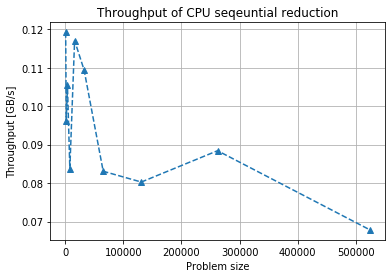
\includegraphics[width=0.7\textwidth]{cpu_sequtential.png}


\subsection{Reduction - GPU parallel initial version}
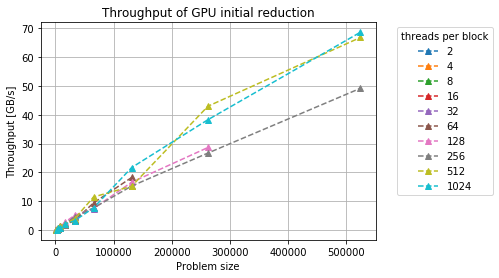
\includegraphics[width=0.9\textwidth]{gpu_initial.png}

\subsection{Reduction - GPU parallel optimized version}
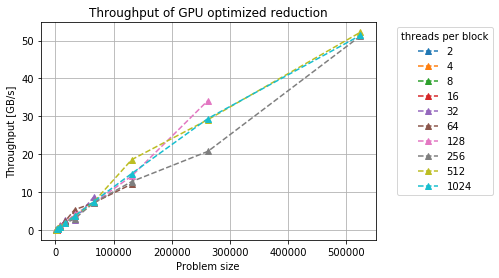
\includegraphics[width=0.9\textwidth]{gpu_optimized.png}

\subsection{Willingness to present}
Hereby, we declare our will to present the results shown in the former sections.


\end{document}